\documentclass[tikz, border=10pt]{standalone}
\usepackage{tikz}
\usetikzlibrary{shapes, shadows, calc, positioning, decorations.markings}

% Define colors
\definecolor{GeoskanBlue}{RGB}{0, 89, 166}
\definecolor{GeoskanOrange}{RGB}{255, 100, 0}
\definecolor{GeoskanBlack}{RGB}{30, 30, 30}
\definecolor{GeoskanSilver}{RGB}{200, 200, 200}
\definecolor{GeoskanLens}{RGB}{50, 50, 80}
\definecolor{GeoskanLED}{RGB}{0, 255, 0}

\begin{document}
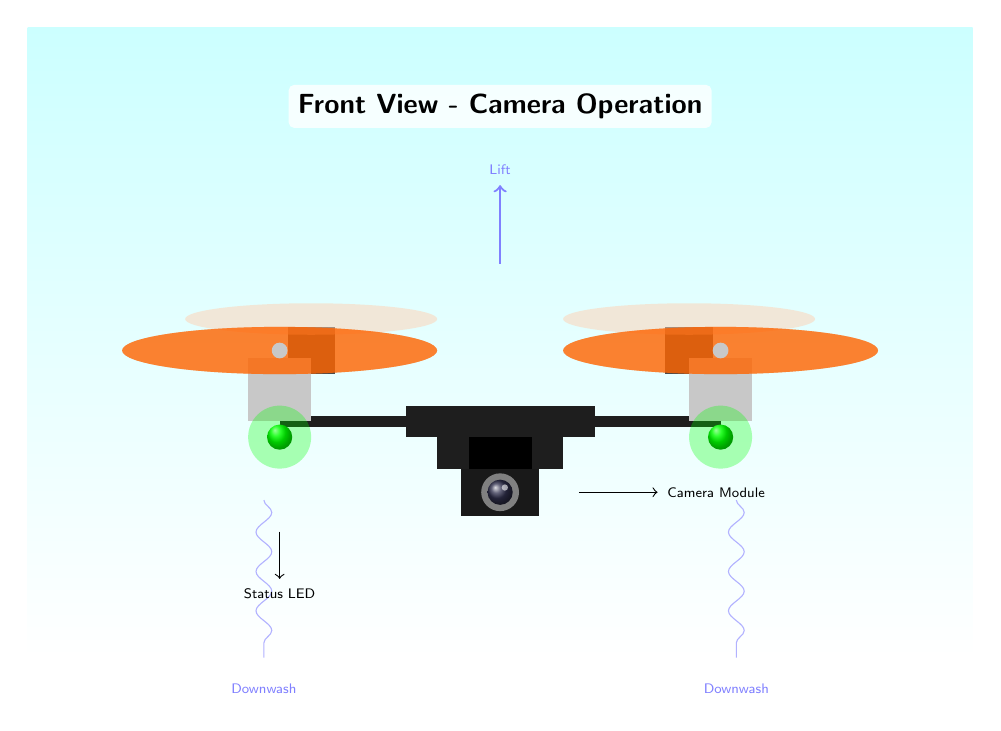
\begin{tikzpicture}[scale=2]

    % --- Background (Sky) ---
    \shade[top color=cyan!20, bottom color=white] (-3, -1) rectangle (3, 3);
    
    % --- Drone Body (Front View Perspective) ---
    % Front Arms (angled towards viewer slightly)
    \def\armAngle{20}
    \def\armLength{1.5}
    
    % Rear Arms (behind, smaller/darker)
    \coordinate (RearLeft) at (-1.2, 0.8);
    \coordinate (RearRight) at (1.2, 0.8);
    
    % Rear Motors
    \fill[GeoskanBlack!80] (RearLeft) ++(-0.15, 0) rectangle ++(0.3, 0.3);
    \fill[GeoskanBlack!80] (RearRight) ++(-0.15, 0) rectangle ++(0.3, 0.3);
    
    % Rear Props (Blurred disk)
    \fill[GeoskanOrange!30, opacity=0.5] (RearLeft) ++(0, 0.35) ellipse (0.8 and 0.1);
    \fill[GeoskanOrange!30, opacity=0.5] (RearRight) ++(0, 0.35) ellipse (0.8 and 0.1);

    % --- Main Frame (Center) ---
    \fill[GeoskanBlack] (-0.6, 0.4) rectangle (0.6, 0.6); % PCB
    \fill[GeoskanBlack] (-0.4, 0.2) rectangle (0.4, 0.4); % Battery Holder
    
    % --- Camera Module (Prominent) ---
    \node[anchor=center] (cam) at (0, 0.1) {};
    % Mount
    \fill[black] (-0.2, 0.2) rectangle (0.2, 0.4);
    % Camera Body
    \fill[black!90] (-0.25, -0.1) rectangle (0.25, 0.2);
    % Lens Ring
    \fill[gray] (0, 0.05) circle (0.12);
    % Lens Glass (Reflection)
    \shade[ball color=GeoskanLens] (0, 0.05) circle (0.08);
    \fill[white, opacity=0.6] (0.03, 0.08) circle (0.02); % Glint
    
    % --- Front Arms ---
    \coordinate (FrontLeft) at (-1.4, 0.5);
    \coordinate (FrontRight) at (1.4, 0.5);
    
    % Arms connecting to center
    \draw[line width=4pt, GeoskanBlack] (-0.6, 0.5) -- (FrontLeft);
    \draw[line width=4pt, GeoskanBlack] (0.6, 0.5) -- (FrontRight);
    
    % --- Front Motors ---
    \fill[GeoskanSilver] (FrontLeft) ++(-0.2, 0) rectangle ++(0.4, 0.4);
    \fill[GeoskanSilver] (FrontRight) ++(-0.2, 0) rectangle ++(0.4, 0.4);
    
    % --- Front Propellers (Spinning) ---
    % Using motion blur effect with multiple ellipses
    \foreach \opacity in {0.2, 0.4, 0.6} {
        \fill[GeoskanOrange, opacity=\opacity] (FrontLeft) ++(0, 0.45) ellipse (1.0 and 0.15);
        \fill[GeoskanOrange, opacity=\opacity] (FrontRight) ++(0, 0.45) ellipse (1.0 and 0.15);
    }
    \fill[GeoskanSilver] (FrontLeft) ++(0, 0.45) circle (0.05); % Nut
    \fill[GeoskanSilver] (FrontRight) ++(0, 0.45) circle (0.05); % Nut

    % --- LED Indicators (Active) ---
    \shade[ball color=GeoskanLED] (FrontLeft) ++(0, -0.1) circle (0.08);
    \shade[ball color=GeoskanLED] (FrontRight) ++(0, -0.1) circle (0.08);
    
    % Glow effect
    \fill[GeoskanLED, opacity=0.3] (FrontLeft) ++(0, -0.1) circle (0.2);
    \fill[GeoskanLED, opacity=0.3] (FrontRight) ++(0, -0.1) circle (0.2);

    % --- Action Lines (Hovering) ---
    \draw[->, thick, blue!50] (0, 1.5) -- (0, 2.0) node[above, font=\sffamily\tiny] {Lift};
    \foreach \x in {-1.5, 1.5} {
        \draw[decorate, decoration={snake, amplitude=1mm, segment length=5mm}, blue!30] (\x, 0) -- (\x, -1);
        \node[blue!50, font=\tiny\sffamily] at (\x, -1.2) {Downwash};
    }

    % --- Labels ---
    \node[font=\bfseries\sffamily, fill=white, opacity=0.8, text opacity=1, rounded corners=2pt] at (0, 2.5) {Front View - Camera Operation};
    \draw[->] (0.5, 0.05) -- (1.0, 0.05) node[right, font=\tiny\sffamily] {Camera Module};
    \draw[->] (-1.4, -0.2) -- (-1.4, -0.5) node[below, font=\tiny\sffamily] {Status LED};

\end{tikzpicture}
\end{document}
